\documentclass[conference]{IEEEtran}
\IEEEoverridecommandlockouts
% The preceding line is only needed to identify funding in the first footnote. If that is unneeded, please comment it out.
\usepackage{amsmath,amsthm,amssymb} %modos matemáticos y  simbolos
\usepackage{latexsym,amsfonts} %simbolos matematicos
\usepackage{cancel} %hacer la linea que cancela las ecuaciones
\usepackage[spanish, es-noshorthands]{babel} %comandos en español y cambia el cuadro por la tabla
\decimalpoint %cambia las comas por puntos decimal
\usepackage[utf8]{inputenc} %caracteristicas del español
\usepackage{physics} %Simbolos fisicos
\usepackage{array} %mejores formatos de tabla
\parindent =0cm %sangria 
\usepackage{algorithmic}
\usepackage{graphicx}
\usepackage{textcomp}
\usepackage{xcolor}
\usepackage{mathtools} 
\usepackage[framemethod=TikZ]{mdframed}%Entornos talegas
\usepackage[colorlinks = true,
			linkcolor = blue,
			citecolor = black,
			urlcolor = blue]{hyperref}%formato de los links y URL's
\usepackage{multicol} %varias columnas
\usepackage{enumerate} %enumeraciones
\usepackage{pgf,tikz,pgfplots} %documentos en formato tikz
\usepackage{mathrsfs} %letras chingonas (transformada de laplace)
\usepackage{subfigure} %varias figuras seguidas
\usepackage{tabulary}
\usepackage{multirow} %ocupar varias filas en una tabla
\usepackage{fancybox} %recuadros talegas
\usepackage{float} %ubicar graficas
\usepackage{color}
\usepackage{comment}
\usepackage{stackrel}
\usepackage{calligra}
\usepackage{lipsum}
\usepackage{cite}
%\pgfplotsset{compat=1.17} 

\newcommand{\R}{\mathbb{R}}
\newcommand{\Z}{\mathbb{Z}}
%%%%%%%%%%%%%%%%%%%%%%%%%%%%%%%%%%%%%%%%%%%%%%%%%%%%%%
\def\BibTeX{{\rm B\kern-.05em{\sc i\kern-.025em b}\kern-.08em
    T\kern-.1667em\lower.7ex\hbox{E}\kern-.125emX}}
\begin{document}



%%% CARÁTULA
\begin{titlepage}



\begin{flushleft}
    Universidad de San Carlos de Guatemala \\
    Escuela de Ciencias Físicas y Matemáticas \\
    Curso: Laboratorio de Instrumentación \\
    Profesor: Wendy Miranda
\end{flushleft}

\vspace{6cm}

\begin{center}
    \huge{Puentes H} \\[1cm]
    \large{Tarea 5}
\end{center}

\vspace{9.75cm}

\begin{flushright}
	Javier de León \\
    $201603068$ \\
    Diego Sarceño \\
    $201900109$
\end{flushright}

\vspace{0.5cm}

\begin{center}
    Guatemala, 11 de noviembre del 2022
\end{center}

\end{titlepage}



\begin{abstract}
    
\end{abstract}

\begin{IEEEkeywords}
    
\end{IEEEkeywords}

\section{Objetivos}

\subsection{General}
    \begin{enumerate}[1.]
        \item Comprender el funcionamiento de la region de corte y saturación de los transistores.
    \end{enumerate}
\subsection{Específicos}
    \begin{enumerate}
        \item Ser capaz de tener un control por medio de transistores utilizados como interruptores.
    \end{enumerate}
%\section{Introducción}
    
\section{Marco Teórico}
Ya tratamos los transistores y diodos en las prácticas pasadas, así que no ahondaremos en describir su funcionamiento, únicamente en el de los puentes $H$.
\subsection{Puentes H}
El puente $H$ es un circuito que permite que un motor de corriente directa pueda girar en ambos sentidos mediante un cambio manual (push bottom, switch, etc.), nombrados así por su característica forma. Su construcción puede variar entre $4$ transistores NPN, $4$ diodos y un interruptor SPDT para enviar corriente y activar diferentes transistores o únicamente switch (Figura \ref{bridge_wiki}) que permitan el paso de corriente cuyo análisis se puede hacer mediante una tabla de verdad.

\begin{figure}[H]
	\centering
	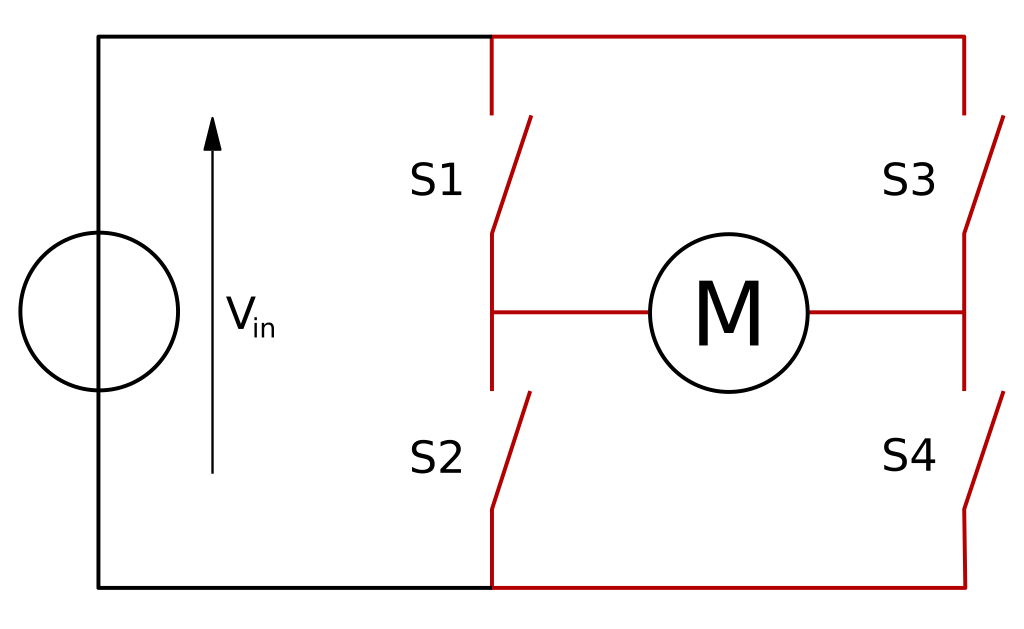
\includegraphics[scale=0.15]{img/bridge_wiki.png}
	\caption{Puente H con switch, imagen extraída de Wikipedia.}
	\label{bridge_wiki}
\end{figure}
Para el circuito de la figura \ref{bridge_wiki}, se tiene la siguiente tabla de verdad
\begin{table}[H]
	\centering
	\caption{Tabla extraída de Wikipedia (Solo se muestran las configuraciones que serán reelvantes en el resto de la práctica).}
	\begin{tabular}{||c|c|c|c||c||}
		\hline
		\hline
		$S_1$ & $S_2$ & $S_3$ & $S_4$ & \textbf{Resultado} \\
		\hline
		\hline
		1 & 0 & 0 & 1 & El motor gira en "avance" \\
		1 & 0 & 0 & 1 & El motor gira en "retroceso" \\
		0 & 0 & 0 & 0 & El motor se detiene bajo su inercia \\
		\hline
		\hline
	\end{tabular}
\end{table}
    
\section{Diseño Experimental}
El circuito simulado sigue el siguiente diagrama
\begin{figure}[H]
	\centering
	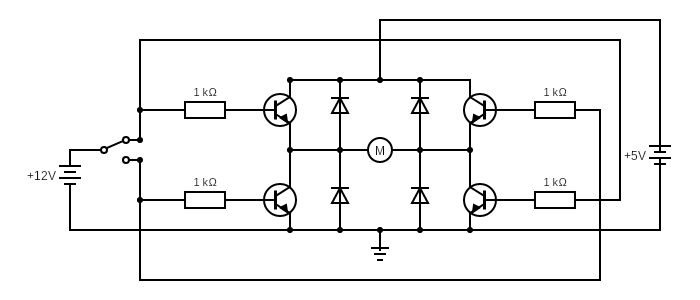
\includegraphics[scale=0.3]{img/bridge_diagram.png}
	\caption{Diagrama del circuito con puente H.}
	\label{bridge_diagram}
\end{figure}
%    \subsection{Materiales a Utilizar}
%        \begin{itemize}
%    	\item 
%    \end{itemize}
%
%    \subsection{Procedimientos}
%        \begin{enumerate}
%            \item 
%        \end{enumerate}
\section{Resultados}
    
\section{Discusión de Resultados}
\begin{enumerate}
    \item 
   
\end{enumerate}
\section{Conclusiones}
\begin{enumerate}
    \item 
\end{enumerate}
%\section{Recomendaciones}

\section{Anexos}
\subsection{Simulación}
Simulación realizada en \textit{TinkerCad}.
\begin{figure}[H]
	\centering
	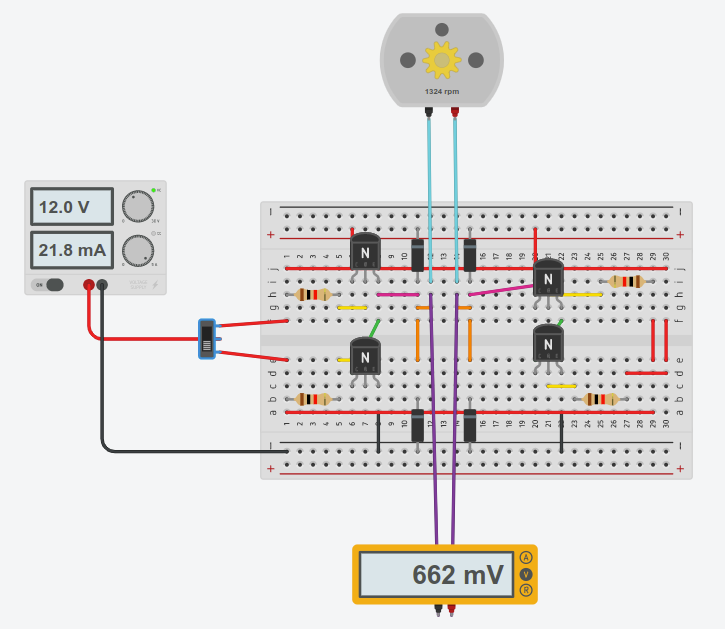
\includegraphics[scale=0.3]{img/bridge_plus_simu.png}
	\caption{Simulación realizada del circuito con puente H con motor girando a favor de las manecillas.}
	\label{bridge_plus_simu}
\end{figure}

\begin{figure}[H]
	\centering
	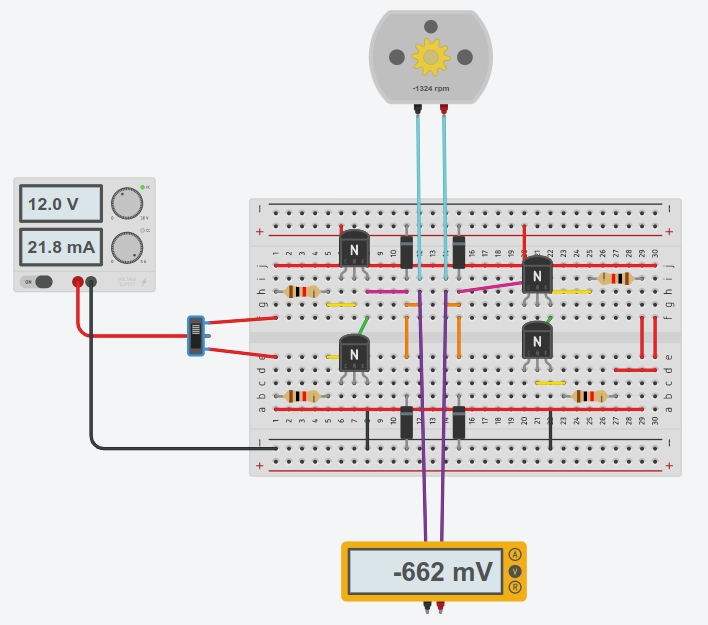
\includegraphics[scale=0.3]{img/bridge_minus_simu.png}
	\caption{Simulación realizada del circuito con puente H con motor girando en contra de las manecillas.}
	\label{bridge_minus_simu}
\end{figure}


\begin{thebibliography}{00}
\bibitem{b1} Donald A. Neamen, 2010. \textit{Microelectronics: Circuit Analysis and Design}. 4th ed. Mc Graw Hill.
\bibitem{b2} 2021. \textit{Circuit Diagram}. \url{https://www.circuit-diagram.org/}
\end{thebibliography}

\end{document}